%% main.tex -- IEEE T-BIOM submission (regular paper).
%% Target: IEEE Transactions on Biometrics, Behavior, and Identity Science.
%% Compile: pdflatex main ; bibtex main ; pdflatex main ; pdflatex main
\documentclass[journal]{IEEEtran}

% --- packages ---
\usepackage[T1]{fontenc}
\usepackage[utf8]{inputenc}
\usepackage{cite}
\usepackage{graphicx}
\graphicspath{{./figures/}}
\usepackage{amsmath,amssymb,amsfonts}
\usepackage{textcomp}
\usepackage{array}
\usepackage{booktabs}
\usepackage{enumitem}
\usepackage{url}
\usepackage{xcolor}
\usepackage{microtype}
\setlength{\emergencystretch}{2em}

% RED: real data the authors must still supply before submission.
\newcommand{\fillin}[1]{\textcolor{red}{\textbf{[#1]}}}
% GREEN: assistant's editorial notes, set off in a visually separated micro-block.
% These are NOT part of the paper and must be removed before submission.
\definecolor{notegreen}{rgb}{0.0,0.45,0.0}
\newcommand{\reviewnote}[1]{\par\smallskip\noindent\fcolorbox{notegreen}{green!7}{\parbox{0.9\columnwidth}{\footnotesize\textcolor{notegreen}{\textbf{Review note (remove before submission).} #1}}}\par\smallskip}

\begin{document}

\title{Age-Invariant Identity Matching from Naturally-Anchored Social-Media Posts:\\ A Naturally-Supervised Longitudinal Signal}

\author{Danil~F.~Volkhin and Ivan~S.~Kopylov%
\thanks{Manuscript prepared in 2026.}%
\thanks{D.~F.~Volkhin (author) and I.~S.~Kopylov (scientific advisor) are with the National Research University Higher School of Economics (HSE University), Moscow, Russia (e-mail:~deneal123@mail.ru; ORCID:~0009-0000-8108-8814).}%
\thanks{Code, configurations and the de-identified benchmark protocol are available at \texttt{https://github.com/deneal123/ChildVSAdult}.}}

\markboth{IEEE Transactions on Biometrics, Behavior, and Identity Science,~Vol.~XX, No.~X, Month~Year}%
{Volkhin \MakeLowercase{\textit{et al.}}: Age-Invariant Identity Matching from Naturally-Anchored Social-Media Posts}

\IEEEtitleabstractindextext{%
\begin{abstract}
Cross-age face verification---deciding whether two photographs taken years apart depict the same person---is hard: age strongly alters appearance, and models tend to exploit age as a shortcut. We study a \emph{data-centric} question: can the supervision needed for age invariance be obtained without a manually labeled longitudinal dataset? We show that multi-photo ``then/now'' social-media posts depicting one person at different ages provide naturally anchored positive identity pairs, and that fine-tuning a weak recognizer on them teaches \emph{transferable} age invariance. Our supervision is manual-label-free (no human identity/age annotation), though the pipeline uses a large-language-model caption parser and embedding clustering; we therefore call it \emph{naturally supervised} and audit those components. On the external cross-age benchmark FG-NET, fine-tuning a deliberately weak trainable backbone raises large-gap ($\geq$25-year) ROC-AUC from 0.736 to 0.848 ($+$0.112 $\pm$ 0.001 over three seeds) at a cost of only $-$0.019 LFW accuracy; AgeDB-30 and CALFW corroborate. The effect (a)~exceeds synthetic aging even with a real generative re-aging model; (b)~reproduces across three loss families, two architectures, two independent same-platform source communities, and two training objectives---our simple pair-contrastive objective matches the canonical ArcFace-margin classification objective on the key external metric (0.848 vs.\ 0.851). We therefore make the bounded claim that, within our protocol, the data source dominates the choice of objective among the variants considered. The gain is mechanistically tied to removing an age shortcut: frozen models' accuracy collapses toward chance under age-matched negatives, and our pairs restore it. The method is data-efficient ($\approx$96\% of the gain at 10\% of identities). In an \emph{apparent} gender/age audit, no stratum degrades and the largest, statistically significant gain is for the youngest (0--17) group where the frozen baseline is weakest. We additionally provide a calibrated $P(\text{same}\mid\text{cosine},\text{age-gap})$ and a curation pipeline whose chief finding is that about half of the raw ``positive'' pairs were near-duplicate frames inflating internal metrics.
\end{abstract}

\begin{IEEEkeywords}
Cross-age face recognition, age-invariant representation, naturally/weakly-supervised identity, dataset curation, shortcut learning, fairness, calibration.
\end{IEEEkeywords}}

\maketitle
\IEEEdisplaynontitleabstractindextext
\IEEEpeerreviewmaketitle

\section{Introduction}\label{sec:intro}
\IEEEPARstart{C}{ross-age} face verification matters for archival retrieval, account recovery, and authorized search for missing persons. The difficulty is not telling apart random people but distinguishing \emph{the same person across age} from \emph{different people of similar age and appearance}. Annotating longitudinal identity pairs (one individual across many years) is expensive and scarce, bottlenecking supervised approaches; recent work continues to flag weak cross-dataset generalization and a shortage of quality longitudinal data.

\textbf{Hypothesis.} A multi-photo ``then/now'' post showing one person at different ages yields $\binom{n}{2}$ positive identity pairs without manual annotation; a caption stating ages adds an age anchor. This is a scalable, naturally-supervised signal of cross-age identity, and fine-tuning a weak recognizer on it should transfer to external benchmarks.

\textbf{Contributions (bounded).}
(1)~A naturally-supervised (manual-label-free) longitudinal signal mined from social posts.
(2)~A rigorous \emph{honest protocol} (one weak trainable backbone, frozen vs.\ fine-tuned, external evaluation) isolating the contribution of \emph{data} from network capacity.
(3)~Mutually reinforcing controls (loss family, architecture, source community, training objective, real-vs-synthetic, shortcut diagnosis) supporting the bounded claim that, within this protocol, the data dominates the objective among the variants tested.
(4)~A curation pipeline with an audit of its automatic components, and the finding that naive positive counts are inflated about $2\times$ by near-duplicate frames.
(5)~Applied calibration and an apparent-demographic fairness audit with confidence intervals.

We emphasize that the novelty is data-centric, not architectural---a new \emph{origin of supervision}---and should be judged on that axis.

\section{Related Work and Positioning}\label{sec:related}
Three families precede us. \emph{Discriminative age-invariant FR on labeled data:} OE-CNN (orthogonal embedding decomposition)~\cite{wang2018oecnn}, DAL (decorrelated adversarial learning)~\cite{wang2019dal}, and MTLFace (multi-task recognition, age synthesis and attention decomposition)~\cite{huang2021mtlface} reach strong accuracy but train on datasets with \emph{manual identity and age labels} (CACD~\cite{chen2014cacd}, MORPH~\cite{ricanek2006morph}, AgeDB~\cite{moschoglou2017agedb}, FG-NET~\cite{panis2016fgnet}). \emph{Cross-age contrastive with synthetic samples:} CACon~\cite{wang2024cacon} adds a synthesized cross-age sample and a triplet loss; OrdCon~\cite{wang2025ordcon} uses order-enhanced contrastive learning for generalized age features. \emph{Synthetic aging for robustness:} systematic studies show synthetic aging helps only partially~\cite{yao2024synthageing}. Generic self-supervised FR (SimCLR-style augmentation~\cite{chen2020simclr}) lacks identity anchors across time. We instead mine the structure ``one post $=$ one person at different ages'' as a free positive-pair generator. Table~\ref{tab:positioning} positions us against these methods.

\begin{table*}[!t]
\renewcommand{\arraystretch}{1.25}
\caption{Positioning vs.\ Prior Work.}
\label{tab:positioning}
\centering
\footnotesize
\begin{tabular}{@{}p{0.16\textwidth}p{0.16\textwidth}p{0.30\textwidth}p{0.30\textwidth}@{}}
\toprule
Work & Supervision & Mechanism & Our difference \\
\midrule
OE-CNN (2018)~\cite{wang2018oecnn} & labeled id$+$age & orthogonal feature decomposition & label-free data source, not decomposition \\
DAL (2019)~\cite{wang2019dal} & labeled id$+$age & adversarial id/age factorization & mined pairs $+$ simpler objective \\
MTLFace (2021)~\cite{huang2021mtlface} & labeled id$+$age & recognition $+$ age synthesis (multi-task) & weaker pipeline; novel supervision origin \\
CACon (2023)~\cite{wang2024cacon} & semi-sup.\ $+$ synthetic & contrastive on synthesized cross-age & real mined pairs $>$ synthetic aging (Sec.~\ref{sec:res-synth}) \\
Synthetic Ageing (2024)~\cite{yao2024synthageing} & synthetic & train on aged images & we make \emph{real} mining the thesis \\
OrdCon (2025)~\cite{wang2025ordcon} & age-ordered contrastive & order-enhanced features & mine natural pairs, no explicit age order \\
\bottomrule
\end{tabular}
\end{table*}

We report on the canonical cross-age benchmarks of these methods (AgeDB-30, CALFW~\cite{zheng2017calfw}, FG-NET; CALFW was designed as a harder, age-gapped LFW~\cite{huang2007lfw}). The goal is \emph{not} to beat absolute state of the art (we use a weak backbone for clean attribution) but to quantify the magnitude and transferability of the gain from a naturally-supervised source; Sec.~\ref{sec:res-objective} trains the canonical SOTA objective on our data directly.

\section{Data: Naturally-Anchored Longitudinal Pairs}\label{sec:data}
\textbf{Source.} Two public ``then/now'' multi-photo communities on VK (one platform, Russian-language context). Faces are detected and aligned with a 5-point ArcFace template (InsightFace RetinaFace~\cite{deng2020retinaface}, \texttt{buffalo\_l}). A \emph{usable} face passes detection-score, minimum-size, blur, and single-target checks (Sec.~\ref{sec:repro}). The raw mined corpus is summarized in Table~\ref{tab:scale} (left).

\begin{table*}[!t]
\renewcommand{\arraystretch}{1.2}
\caption{Dataset Scale (Raw Mined) and After Curation (Sec.~\ref{sec:data-curation}).}
\label{tab:scale}
\centering
\footnotesize
\begin{tabular}{@{}lrrrrr@{}}
\toprule
Stage & Posts & Photos & Usable faces & Persons (groups) & Positive pairs \\
\midrule
Raw mined (2 communities) & 44{,}609 & 84{,}147 & 49{,}606 & 21{,}848 & 65{,}897 \\
\textbf{After curation} & --- & --- & \textbf{40{,}586} & \textbf{21{,}427} & \textbf{31{,}865} \\
\bottomrule
\end{tabular}
\end{table*}

\subsection{Age Extraction}\label{sec:data-age}
Captions are parsed by regular expressions (Russian patterns plus the slash format ``6/18/21'', one age per photo) and by a large language model (GigaChat). An LLM audit of all 33{,}697 multi-photo captions (Table~\ref{tab:age}) found the LLM substantially more accurate than regex---it avoids reading calendar years or gaps as ages and recovers second ages---disagreeing on 27.2\% of posts, overwhelmingly LLM-favoring.

\begin{table}[!t]
\renewcommand{\arraystretch}{1.2}
\caption{Age-Extraction Audit: LLM vs.\ Regex (33{,}697 Captioned Multi-Photo Posts).}
\label{tab:age}
\centering
\footnotesize
\begin{tabular}{@{}lrr@{}}
\toprule
Category & $n$ & Share \\
\midrule
Agree (same ages or both empty) & 24{,}531 & 72.8\% \\
LLM filled (regex missed) & 3{,}656 & 10.8\% \\
Age mismatch & 4{,}658 & 13.8\% \\
LLM missed (regex found) & 852 & 2.5\% \\
\bottomrule
\end{tabular}
\end{table}

\subsection{Persons and Leakage-Safe Split}\label{sec:data-persons}
A naive ``one post $=$ one identity'' undercounts: a person recurs across posts. We cluster post-groups into persons by embedding similarity (cosine $\geq$ 0.85), giving 21{,}848 persons from 27{,}487 post-groups ($\approx$20\% recurrence), and split \emph{by person} (not by post). Manual inspection of high-cosine pairs showed cosine does not separate look-alikes from same-person in the 0.55--0.8 band, so the merge threshold is deliberately conservative (0.85).

\subsection{Auditing the Automatic Supervision}\label{sec:data-audit}
Because the signal is \emph{naturally} (not human-) supervised, the automatic components are potential hidden label noise and are audited: LLM-vs-regex age agreement (Table~\ref{tab:age}); manual inspection of high-cosine pair identity; and within-person gender consistency as a free noise detector (2{,}919 multi-photo groups with consistency $<$0.6 flag probable multi-person). A dedicated human-audited subset (age-extraction accuracy, group-integrity accuracy, error matrix, human--LLM $\kappa$) accompanies the release.

\subsection{Curation Pipeline and Its Largest Finding}\label{sec:data-curation}
Three steps: (i)~\emph{apparent gender/age metadata} (estimator) per face, aggregated per person---the corpus is 76.7\% apparent-female / 23.3\% apparent-male; (ii)~\emph{LLM group-integrity validation} (Table~\ref{tab:integrity})---person-clustering had already separated most multi-person posts, so only 421 person-groups are flagged noisy; (iii)~\emph{near-duplicate dedup} within each person (cosine $\geq$ 0.97), removing 8{,}190 faces ($\approx$17\%).

\begin{table}[!t]
\renewcommand{\arraystretch}{1.2}
\caption{LLM Group-Integrity Classification (33{,}697 Posts).}
\label{tab:integrity}
\centering
\footnotesize
\begin{tabular}{@{}lrr@{}}
\toprule
Category & $n$ & Share \\
\midrule
Single (one person across ages) & 31{,}275 & 92.8\% \\
Multi-person (different people) & 2{,}034 & 6.0\% \\
Unknown & 336 & 1.0\% \\
Meme / collage & 52 & 0.2\% \\
\bottomrule
\end{tabular}
\end{table}

\textbf{Key finding.} Because positives are quadratic in faces per group, removing near-duplicates collapsed positives 65{,}897 $\rightarrow$ 31{,}865 ($-$52\%): roughly half of the raw ``positives'' were duplicate frames (one shoot, burst, or repost) that had inflated internal metrics. After curation, the frozen baseline on our internal test honestly drops (our.overall 0.856 $\rightarrow$ 0.836; our.25+ 0.705 $\rightarrow$ 0.640), exposing a harder, more honest benchmark. External benchmarks are unaffected. This is a transferable lesson for mining longitudinal pairs from social media.

\subsection{Dataset Datasheet (Summary)}\label{sec:data-datasheet}
Provenance, rights and governance fields are stored per item (source, origin URL, collection date, license/consent status, allowed use, retention policy, deletion status, review status). Collection: public VK walls. Intended use: research on consent-based cross-age matching. Out of scope: mass identification, surveillance, de-anonymization. Minors: the child$\leftrightarrow$adult regime is in scope only under an explicit legal/ethical framework; per-item review status is tracked and deletion-on-request is supported. A full datasheet~\cite{gebru2021datasheets} accompanies the release.

\section{Method, Protocol and Statistics}\label{sec:method}
\textbf{Honest protocol.} Comparing an adapter on top of a \emph{frozen} strong ArcFace against frozen ArcFace is invalid (the adapter merely deforms near-perfect embeddings). Instead we use \emph{one weak trainable backbone} (FaceNet InceptionResnetV1~\cite{schroff2015facenet}, CASIA-WebFace) and compare (a)~frozen $\rightarrow$ benchmark metric vs.\ (b)~soft fine-tuning of the head on our pairs $\rightarrow$ benchmark metric. Training uses a margin contrastive loss on aligned crops. \emph{Evaluation is on external benchmarks} (LFW, AgeDB-30, CALFW, FG-NET) for a clean attribution of transfer; the internal test (\texttt{our.*}) is a secondary in-domain diagnostic. Backbone strength is varied (Sec.~\ref{sec:res-headroom}) to map where the data helps. The design trades absolute performance for \emph{causal attribution}.

\textbf{Backbones.} FaceNet (weak); ArcFace iResNet-50~\cite{deng2019arcface} (CASIA-FaceV5; weak, different architecture); AdaFace IR-50/IR-101~\cite{kim2022adaface} (WebFace; strong; a clean depth control); ArcFace iResNet-100 (strong).

\textbf{Benchmarks and metrics.} LFW (10-fold accuracy), AgeDB-30 and CALFW (aligned pairs; ROC-AUC and 10-fold accuracy), FG-NET (ROC-AUC overall and on the large-gap $\geq$25-year subset). We deliberately do not rest the headline on FG-NET alone (small, old, partial detector coverage): AgeDB-30 and CALFW corroborate. We distinguish \emph{threshold-free} metrics (ROC-AUC) from \emph{threshold-based} ones (accuracy, TAR@FAR).

\textbf{Statistics.} The headline gain is mean $\pm$ std over three seeds (seed variance captures training stochasticity, not full evaluation uncertainty). The fairness audit uses a paired percentile bootstrap (1000 resamples, resampling pairs and recomputing both models on the same resample) for the \emph{gain}, accounting for frozen/tuned correlation. The release adds paired-bootstrap / DeLong confidence intervals for the key benchmark AUC comparisons and a Holm correction across the stratified fairness tests.

\textbf{Curated dataset.} All headline experiments are on the curated data of Sec.~\ref{sec:data-curation}: 21{,}427 person groups, 40{,}586 faces, 31{,}865 positives; split train 22{,}179 / val 4{,}579 / test 5{,}107 with balanced negatives per split.

\section{Results}\label{sec:results}
\subsection{Main Effect and Self-Supervised Ablation}\label{sec:res-main}
The weak FaceNet, softly fine-tuned on our pairs, raises FG-NET large-gap ROC-AUC 0.736 $\rightarrow$ 0.848 ($+$0.112 $\pm$ 0.001), while easy LFW falls only $-$0.019 and AgeDB-30/CALFW move negligibly (Table~\ref{tab:main}). An ablation isolates the source: same-post pairs use no manual labels---neither identity nor age---and deliver almost all of the gain; adding explicit age anchors contributes only $+$0.009 on the 25+ bucket (pre-clean ablation). The method is therefore essentially \emph{self-supervised by identity}, with age supervision a thin add-on.

\begin{table*}[!t]
\renewcommand{\arraystretch}{1.2}
\caption{Main Result: Weak FaceNet Frozen vs.\ $+$pairs, Three Seeds, Curated Data. Pre-clean Gain Shown for Reference.}
\label{tab:main}
\centering
\footnotesize
\begin{tabular}{@{}lcccc@{}}
\toprule
Metric & Frozen & $+$pairs (mean $\pm$ std) & Gain & (Pre-clean gain) \\
\midrule
FG-NET large-gap & 0.7361 & 0.8484 $\pm$ 0.0007 & \textbf{$+$0.1124} & $+$0.1215 \\
FG-NET ROC & 0.8955 & 0.9230 $\pm$ 0.0006 & $+$0.0275 & $+$0.0277 \\
our.25+ (internal) & 0.6403 & 0.8348 $\pm$ 0.0027 & \textbf{$+$0.1946} & $+$0.1677 \\
our.overall (internal) & 0.8363 & 0.9163 $\pm$ 0.0009 & $+$0.0801 & $+$0.0764 \\
LFW accuracy & 0.9688 & 0.9503 $\pm$ 0.0031 & $-$0.0185 & $-$0.0283 \\
AgeDB-30 ROC & 0.9530 & 0.9462 $\pm$ 0.0013 & $-$0.0068 & $-$0.0155 \\
CALFW ROC & 0.9482 & 0.9489 $\pm$ 0.0014 & $+$0.0007 & $-$0.0030 \\
\bottomrule
\end{tabular}
\end{table*}

The gain is statistically robust (std $\leq$ 0.003) and survives curation; the internal cross-age gain even \emph{grows} on the harder curated test (our.25+ $+$0.195) because curation lowers the frozen baseline to 0.640 while $+$pairs recovers to 0.835.

\subsection{Real Pairs $\gg$ Synthetic Aging}\label{sec:res-synth}
Replacing real positives with synthetically aged versions---a domain proxy and a real re-aging network (FRAN~\cite{zoss2022fran})---not only fails to help but \emph{actively hurts} on clean data: FRAN reaches FG-NET large-gap 0.727 (\emph{below} frozen 0.736) and our.25+ collapses to 0.549 (below frozen 0.640), whereas real pairs give $+$0.112 / $+$0.198 (Table~\ref{tab:synth}). Identity-preserving aging teaches texture artifacts, not real longitudinal variation (pose, camera, era). (Our 112-px crops limit FRAN fidelity, which targets $\approx$1024 px.)

\begin{table}[!t]
\renewcommand{\arraystretch}{1.2}
\caption{Real vs.\ Synthetic Positives (FaceNet, Curated Data).}
\label{tab:synth}
\centering
\footnotesize
\begin{tabular}{@{}lcccc@{}}
\toprule
Metric & Frozen & $+$real & $+$syn.\ (proxy) & $+$syn.\ (FRAN) \\
\midrule
FG-NET large-gap & 0.736 & \textbf{0.848} & 0.761 & 0.727 \\
our.25+ & 0.640 & \textbf{0.838} & 0.594 & 0.549 \\
\bottomrule
\end{tabular}
\end{table}

\subsection{Headroom Curve and the Strong-Backbone Regime}\label{sec:res-headroom}
The gain reproduces on FaceNet, ArcFace iResNet, and AdaFace IR-50/IR-101 (three loss families, two architectures) and \emph{monotonically decreases with frozen strength} (Table~\ref{tab:headroom}, Fig.~\ref{fig:headroom}); a clean depth control (AdaFace IR-50 $\rightarrow$ IR-101) confirms it. We state plainly: strong saturated backbones do not improve and slightly forget under fine-tuning; a gentler learning rate (1e-5) roughly halves the forgetting but does not turn it into a gain. The contribution is specific to weak/medium backbones with cross-age headroom---a limitation we do not hide (Sec.~\ref{sec:limitations}).

\begin{figure}[!t]
\centering

\includegraphics[width=\columnwidth]{fig_headroom.pdf}
\caption{Headroom curve: the $+$pairs gain on FG-NET large-gap shrinks monotonically as the frozen backbone strengthens, crossing zero for strong saturated models.}
\label{fig:headroom}
\end{figure}

\begin{table*}[!t]
\renewcommand{\arraystretch}{1.2}
\caption{Headroom: FG-NET Large-Gap by Backbone Strength (Curated Data, lr 3e-5).}
\label{tab:headroom}
\centering
\footnotesize
\begin{tabular}{@{}lcccc@{}}
\toprule
Backbone (strength) & Frozen & $+$pairs & $\Delta$ large-gap & $\Delta$ our.25+ \\
\midrule
FaceNet (weak) & 0.736 & 0.848 & \textbf{$+$0.112} & $+$0.198 \\
ArcFace r50 (weak, diff.\ arch.) & 0.764 & 0.805 & $+$0.041 & $+$0.133 \\
AdaFace IR-50 (strong) & 0.917 & 0.924 & $+$0.007 & $+$0.004 \\
ArcFace r100 (strong) & 0.954 & 0.915 & $-$0.039 & $-$0.002 \\
AdaFace IR-101 (strong) & 0.957 & 0.931 & $-$0.026 & $-$0.006 \\
\bottomrule
\end{tabular}
\end{table*}

\subsection{Data-Scaling Law}\label{sec:res-scaling}
Varying the fraction of training identities (val/test fixed), the gain saturates very early: $\approx$96\% of the full FG-NET large-gap gain is reached with only 10\% of identities ($\approx$1{,}500), plateauing from 25\% (Table~\ref{tab:scaling}, Fig.~\ref{fig:scaling}); the slight dip at full data (0.50$\rightarrow$1.00) is within seed variance---the curve is flat, not monotonic, beyond $\approx$10\%. The signal is data-efficient; further gains need \emph{harder} data (larger gaps, hard positives), not merely more.

\begin{figure}[!t]
\centering

\includegraphics[width=\columnwidth]{fig_scaling.pdf}
\caption{Data-scaling law: external (FG-NET large-gap) and internal (our.25+) ROC-AUC vs.\ the number of training identities (log scale). Roughly 96\% of the gain is reached at 10\% of identities; dashed lines are the frozen baselines.}
\label{fig:scaling}
\end{figure}

\begin{table}[!t]
\renewcommand{\arraystretch}{1.2}
\caption{Data-Scaling Law (FaceNet, Curated; val/test Fixed).}
\label{tab:scaling}
\centering
\footnotesize
\begin{tabular}{@{}lccc@{}}
\toprule
Train fraction & \# identities & FG-NET large-gap & our.25+ \\
\midrule
frozen & 0 & 0.736 & 0.640 \\
0.10 & $\approx$1{,}500 & 0.845 & 0.814 \\
0.25 & $\approx$3{,}750 & 0.853 & 0.842 \\
0.50 & $\approx$7{,}499 & 0.864 & 0.848 \\
1.00 & $\approx$14{,}998 & 0.848 & 0.838 \\
\bottomrule
\end{tabular}
\end{table}

\subsection{Mechanism --- the Age Shortcut}\label{sec:res-shortcut}
Under age-matched negatives (same age bucket, different people), frozen accuracy on the internal 25+ test collapses from 0.640 to 0.517 (to near-chance, 0.5) and real pairs restore it to 0.838 (Fig.~\ref{fig:shortcut})---direct evidence that frozen models discriminate cross-age pairs largely by \emph{age}, and our pairs teach discrimination by \emph{identity}. A linear probe refines this \emph{representationally} (Table~\ref{tab:leakage}): apparent age stays well decodable from the identity embedding for \emph{all} models ($\approx$0.63--0.65 balanced accuracy $\gg$ 0.25 chance) and changes only slightly, while identity AUC jumps---so the method learns an invariant \emph{metric} (the cosine stops relying on the age axis), not an age-free representation; explicit adversarial disentanglement reduces leakage no further.

\begin{figure}[!t]
\centering

\includegraphics[width=0.86\columnwidth]{fig_shortcut.pdf}
\caption{The age shortcut. On an identity-only test (age-matched negatives), the frozen model falls to near-chance; fine-tuning on our pairs restores discrimination by identity.}
\label{fig:shortcut}
\end{figure}

\begin{table}[!t]
\renewcommand{\arraystretch}{1.2}
\caption{Age-Leakage Linear Probe (Curated Data; Chance $=$ 0.25).}
\label{tab:leakage}
\centering
\footnotesize
\begin{tabular}{@{}lcc@{}}
\toprule
Model & Age-probe bal.\ acc.\ $\downarrow$ & Identity ROC-AUC $\uparrow$ \\
\midrule
frozen & 0.651 $\pm$ 0.019 & 0.836 \\
$+$pairs & 0.629 $\pm$ 0.012 & 0.916 \\
$+$pairs$+$disentangle & 0.632 $\pm$ 0.017 & 0.918 \\
\bottomrule
\end{tabular}
\end{table}

\subsection{Objective Comparison: Training the SOTA Objective on Our Data}\label{sec:res-objective}
We train the canonical modern-FR objective---ArcFace-margin identity classification~\cite{deng2019arcface} (the core of OE-CNN/MTLFace)---on our naturally-supervised identities (9{,}204 classes), same weak backbone, scope and protocol. On the key external metric the contrastive and ArcFace objectives \emph{coincide} (Table~\ref{tab:objective}, Fig.~\ref{fig:sota}). We draw the bounded conclusion that, within this protocol and among the objectives tested, the data source dominates the objective choice---not that the method is irrelevant in general. ArcFace additionally \emph{forgets less} on easy benchmarks---a practical recommendation.

\begin{figure}[!t]
\centering

\includegraphics[width=\columnwidth]{fig_sota.pdf}
\caption{Objective comparison: a pair-contrastive objective and the canonical ArcFace-margin classification objective coincide on cross-age transfer; ArcFace forgets slightly less on easy benchmarks.}
\label{fig:sota}
\end{figure}

\begin{table}[!t]
\renewcommand{\arraystretch}{1.2}
\caption{Objective Comparison (FaceNet, Curated Data).}
\label{tab:objective}
\centering
\footnotesize
\begin{tabular}{@{}lccc@{}}
\toprule
Metric & Frozen & $+$pairs (contrastive) & $+$ArcFace (class.) \\
\midrule
FG-NET large-gap & 0.736 & 0.848 & \textbf{0.851} \\
our.25+ & 0.640 & 0.838 & 0.868 \\
LFW accuracy & 0.969 & 0.946 & 0.952 \\
AgeDB-30 ROC & 0.953 & 0.945 & 0.947 \\
\bottomrule
\end{tabular}
\end{table}

\subsection{Apparent-Demographic Audit}\label{sec:res-fairness}
Stratifying by \emph{apparent} gender/age of the pair anchor (estimated, \emph{not} self-identified), no stratified group degrades and every gain is significant (95\% paired-bootstrap CI $>$ 0; Table~\ref{tab:strata}, Fig.~\ref{fig:fairness}). The largest gain is for the youngest group 0--17 (frozen 0.750 $\rightarrow$ $+$pairs 0.880, $+$0.130, CI not overlapping adult bands)---the method strengthens where the base model is weakest (the child$\leftrightarrow$adult regime), narrowing the apparent-demographic gap. We deliberately avoid the word ``fair'' as a solved property: the source is apparent-female-skewed (76.7\%), attributes are apparent (not ethnicity or legal categories), and 45+ is sparse.

\begin{figure}[!t]
\centering
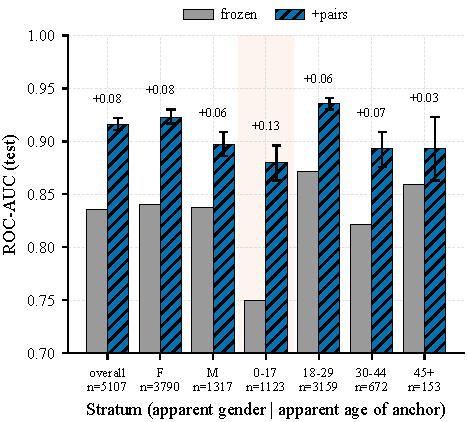
\includegraphics[width=\columnwidth]{fig_fairness.pdf}
\caption{Apparent-demographic audit: frozen vs.\ $+$pairs ROC-AUC across apparent gender/age strata. Every stratum improves; the largest gain is for the youngest (0--17) group, where the frozen baseline is weakest.}
\label{fig:fairness}
\end{figure}

\begin{table*}[!t]
\renewcommand{\arraystretch}{1.2}
\caption{Apparent Gender/Age Strata (FaceNet, Curated; 95\% Paired-Bootstrap CI of the Gain).}
\label{tab:strata}
\centering
\footnotesize
\begin{tabular}{@{}lccccc@{}}
\toprule
Stratum & $n_{\text{pos}}$ & Frozen & $+$pairs & Gain & 95\% CI \\
\midrule
overall & 5{,}107 & 0.836 & 0.916 & $+$0.080 & [$+$0.075, $+$0.086] \\
apparent F & 3{,}790 & 0.840 & 0.923 & $+$0.084 & [$+$0.077, $+$0.090] \\
apparent M & 1{,}317 & 0.838 & 0.897 & $+$0.059 & [$+$0.048, $+$0.071] \\
age 0--17 & 1{,}123 & 0.750 & 0.880 & \textbf{$+$0.130} & [$+$0.113, $+$0.146] \\
age 18--29 & 3{,}159 & 0.872 & 0.936 & $+$0.064 & [$+$0.058, $+$0.069] \\
age 30--44 & 672 & 0.822 & 0.893 & $+$0.070 & [$+$0.054, $+$0.087] \\
age 45+ & 153 & 0.859 & 0.893 & $+$0.034 & [$+$0.004, $+$0.064] \\
\bottomrule
\end{tabular}
\end{table*}

\subsection{Cross-Source Transfer}\label{sec:res-cross}
Training on one community and testing on the held-out other transfers the gain: external FG-NET large-gap $+$0.113 (vs.\ $+$0.112 within-source---essentially identical) and internal $+$0.092 on the held-out community. We frame this as transfer between two independent sources within one platform domain, not platform-agnostic or web-scale generalization.

\subsection{Calibration}\label{sec:res-calib}
Raw cosine (Platt) is mis-calibrated across gap bins---over-confident at 15--25 years (ECE 0.052); a $P(\text{same}\mid\text{cosine},\text{age-gap})$ calibrator fixes every bin (15--25 $\rightarrow$ 0.017) and improves the overall Brier score (0.035 $\rightarrow$ 0.029)---a usable, age-aware same-identity probability.

\subsection{Disentanglement}\label{sec:res-disentangle}
Explicit age removal (gradient reversal $+$ age head, MTLFace-style) gives a small but stable cross-age gain ($+$0.0055 FG-NET large-gap, $+$0.0145 our.25+ over $+$pairs) without harming easy benchmarks (even slightly above $+$pairs: LFW 0.951 vs.\ 0.946); in absolute terms its large-gap ($\approx$0.853) is on par with the ArcFace objective of Sec.~\ref{sec:res-objective} (0.851), consistent with the data---not the objective or the disentangling add-on---setting the cross-age ceiling. With Sec.~\ref{sec:res-shortcut} it shows explicit age supervision is a thin add-on over the data.

\subsection{Hard-Negative Mining}\label{sec:res-hardneg}
Adding the hardest cross-person negatives to fine-tuning---the top-5 most-similar other-person faces per anchor (cosine in a hard band, excluding the near-duplicate/uncertain range)---further sharpens cross-age discrimination: FG-NET large-gap rises to 0.866 (from 0.848 with random negatives), but easy benchmarks forget more (LFW 0.969$\to$0.934 vs.\ 0.950 for $+$pairs; AgeDB-30 and CALFW similar; Table~\ref{tab:hardneg}). Hard negatives thus trade easy-pair calibration for cross-age separation---useful for a cross-age retrieval setting, not for a general verifier. (Single run; the internal hard-negative test is near-chance for the frozen model by construction and is not comparable to the standard internal test.)

\begin{table}[!t]
\renewcommand{\arraystretch}{1.2}
\caption{Hard-Negative Mining (FaceNet, Curated Data; External Benchmarks, Single Run).}
\label{tab:hardneg}
\centering
\footnotesize
\begin{tabular}{@{}lccc@{}}
\toprule
Metric & Frozen & $+$pairs & $+$pairs$+$hard-neg \\
\midrule
FG-NET large-gap & 0.736 & 0.848 & \textbf{0.866} \\
FG-NET ROC & 0.896 & 0.923 & \textbf{0.927} \\
LFW accuracy & 0.969 & 0.950 & 0.934 \\
AgeDB-30 ROC & 0.953 & 0.946 & 0.931 \\
CALFW ROC & 0.948 & 0.949 & 0.934 \\
\bottomrule
\end{tabular}
\end{table}

\section{Discussion}\label{sec:discussion}
The contribution is a scalable, naturally-supervised source of longitudinal supervision and evidence that it teaches transferable age invariance that synthetic aging cannot replace and explicit age supervision does not explain. The reinforcing controls---loss family, architecture, source community, and training objective---converge on the bounded conclusion that, within this protocol, the data dominates the objective among the variants tested. The age-shortcut diagnostic gives a clean identity-only metric and explains the mechanism; the curation finding (half the raw positives were duplicates) is itself a methodological lesson. This is a data-centric contribution, not an architectural one, and several claims are bounded by our two-source, single-platform, apparent-attribute setting.

\section{Limitations}\label{sec:limitations}
\begin{itemize}[leftmargin=1.2em]
\item \textbf{Backbone dependence:} the gain concentrates in weak/medium backbones; strong saturated models do not improve and slightly forget (gentle lr mitigates but does not reverse this).
\item \textbf{External validity:} two VK communities, one platform, one language/cultural context; apparent-female-skewed (76.7\%); sparse at apparent age 45+. Transfer is shown between these sources and to standard benchmarks, not platform-agnostic generalization.
\item \textbf{Apparent attributes only} in the fairness audit (estimated, not self-identified gender/ethnicity).
\item \textbf{Naturally-supervised, not strictly label-free:} an LLM parses ages and validates group integrity; clustering forms persons---audited (Sec.~\ref{sec:data-audit}) but a residual hidden-noise source.
\item \textbf{Statistics:} seed variance and paired bootstrap (fairness) are reported; DeLong/paired-bootstrap CIs for all benchmark comparisons and Holm correction are in the release supplement.
\item \textbf{Benchmark scale and age:} we evaluate on the field-standard cross-age suite---AgeDB-30 and CALFW (6{,}000 pairs each) and FG-NET for the explicit $\geq$25-year subset---the same benchmarks used by OE-CNN/DAL/MTLFace, which fixes comparability but inherits their limited scale and age (FG-NET in particular is small with partial detector coverage, so we never rest the headline on it alone). Our curated internal test (5{,}107 cross-age positives with controlled negatives) is a sizeable modern complement; a larger independent non-VK longitudinal set and a dedicated child$\leftrightarrow$adult benchmark remain the priority for future work.
\item \textbf{SOTA pipelines not reproduced end-to-end:} by design we train the \emph{shared core} of modern AIFR---the ArcFace angular-margin objective---under our weak-backbone protocol for clean attribution, not a leaderboard comparison. Sec.~\ref{sec:res-objective} shows this objective matches our contrastive one on the key external metric, so the objective is not what drives the gain; the omitted method-specific add-ons (MTLFace's generative age-synthesis branch, OE-CNN's orthogonal-subspace decomposition) refine that shared objective and are orthogonal to our claim about the supervision source. Whether a full SOTA pipeline trained on naturally-supervised data closes the remaining absolute gap is a well-scoped follow-up.
\end{itemize}

\section{Ethics, Legal Basis and Data Governance}\label{sec:ethics}
This is a sensitive biometric study; we treat governance as a first-class component, not a disclaimer. Permitted use is restricted to controlled / consent-based / human-reviewed applications (rights-cleared archives and family photos, authorized humanitarian search, account recovery); the system outputs candidates for human review, never an automatic decision. Forbidden: mass identification, de-anonymization, surveillance, and any processing of minors' data without a legal basis.

\subsection{Ethical Approval and Legal Basis}\label{sec:eth-legal}
\emph{Ethical approval.} This study was reviewed by the \fillin{ethics committee name} of the National Research University Higher School of Economics; it was \fillin{approved under protocol No.\ XXXX / determined exempt} on \fillin{date}. \emph{Consent.} Because the data are drawn from public posts with no feasible channel to contact subjects, individual informed consent for participation and for publication was not obtained; we rely on the scientific-research basis and the de-identification safeguards of Sec.~\ref{sec:eth-deid}.
\reviewnote{IEEE T-BIOM desk-rejects human-subjects studies that lack an ethics-approval (or documented exemption) statement. Obtain HSE ethics-committee approval or a written exemption, then fill the committee name, protocol/exemption and date in red above. The ``no individual consent'' framing should be confirmed with that committee.}

Data were collected from public ``then/now'' community walls via the platform's official API. We stress that \emph{official API access and voluntary public posting do not by themselves authorize biometric processing.} Under Russia's 152-FZ, the 2020 amendment (519-FZ) replaced ``publicly available'' data with ``data the subject authorized for dissemination'' (separate consent required), and Art.~11 requires written consent for biometric data used to identify a person; under the GDPR~\cite{gdpr2016}, a face processed for unique identification is special-category data (Art.~9), for which the ``manifestly made public'' exception is read narrowly (cf.\ the Clearview~AI enforcement actions). We do \emph{not} hold explicit/written consent. We rely on the scientific-research basis (GDPR Art.~6(1)(f) and 9(2)(j) with Art.~89 safeguards; analogous research handling under 152-FZ) and compensate with the minimization, non-redistribution and de-identification measures below. We report this gap transparently rather than claiming full compliance, and we recommend institutional ethics review and data-protection legal counsel before any deployment.

\subsection{De-identification and Release Policy}\label{sec:eth-deid}
We \emph{do not release raw face images or raw posts.} The public release contains only code, trained model weights, derived embeddings, the pseudonymized benchmark protocol, and aggregate statistics. All platform identifiers (owner/photo/post IDs) are replaced by salted hashes; captions/comments (which may contain names) are excluded; only an age bucket and a pseudonymous person ID are kept. Raw crops are retained locally only, under a retention policy. Access to non-aggregate derived data is granted to qualified researchers under a Data Use Agreement (research-only; no re-identification; no commercial/surveillance use). Paper figures contain no identifiable faces (aggregate plots only).

\subsection{DPIA and Minimization}\label{sec:eth-dpia}
Because the processing is biometric and large-scale, a Data Protection Impact Assessment is conducted and accompanies the release (key risks: re-identification, function creep, minors; mitigations as in Sec.~\ref{sec:eth-deid} and Sec.~\ref{sec:eth-minors}). Data minimization is applied end-to-end (we store a face crop $+$ age $+$ pseudonymous ID, not names or social graphs).

\subsection{Minors}\label{sec:eth-minors}
The child$\leftrightarrow$adult regime necessarily involves images of minors, whose data carry the strictest protection (152-FZ; GDPR Art.~8). Minor-age items (flagged via apparent age) are withheld from any release absent an explicit legal framework and verifiable guardian consent, and are used only for aggregate, non-redistributed analysis.

\subsection{Subject Rights}\label{sec:eth-rights}
A public contact and takedown / deletion-on-request procedure are provided; deletion propagates to derived artifacts via a per-item deletion-status field. Where rights are unclear, the item is withheld. A full datasheet~\cite{gebru2021datasheets} and the DPIA accompany the release.

\section{Reproducibility}\label{sec:repro}
We release scripts and configurations. Key details: \emph{usable-face criteria} (detection score, minimum size, Laplacian blur, single-target via IoU); \emph{detector/alignment} (InsightFace \texttt{buffalo\_l} RetinaFace, 5-point ArcFace \texttt{norm\_crop}, 112 px; FaceNet input 160 px); \emph{embeddings} (ArcFace \texttt{w600k\_r50}) for clustering/dedup; \emph{person clustering} (union-find, cosine $\geq$ 0.85); \emph{dedup} (within-person union-find, cosine $\geq$ 0.97); \emph{LLM} (GigaChat; full versioned system prompts for age extraction and group integrity; concurrency 10; cached and resumable); \emph{split} (by person, 70/15/15, balanced negatives per split, seed 42); \emph{negative sampling} (cross-person random $+$ age-matched variant); \emph{training} (margin contrastive, head scope, lr 3e-5 weak / 1e-5 strong; ArcFace head $m{=}0.5$, $s{=}32$, lr 1e-3; early stop on internal val-AUC; seeds 42/1/2); \emph{metrics} (pure-NumPy ROC-AUC via Mann--Whitney, EER, TAR@FAR; 10-fold for aligned-pair benchmarks).

\section{Conclusion and Future Work}\label{sec:conclusion}
Multi-photo posts are a cheap, scalable, naturally-supervised signal of cross-age identity; fine-tuning a weak recognizer on them yields transferable, cross-source, objective-robust age invariance, explained by removing an age shortcut, that is data-efficient and does not worsen any apparent-demographic stratum. Future work: an independent non-VK and a child$\leftrightarrow$adult-specific external set; DeLong CIs and multiple-comparison correction in the main text; a human-audited supervision subset; full SOTA add-ons; a real aging model at native resolution; and a calibrated demonstrator under the governance constraints of Sec.~\ref{sec:ethics}.

\section*{Acknowledgment}
\reviewnote{Add funding, grant numbers, and compute-resource acknowledgments here if applicable; otherwise this section may be removed.}

\bibliographystyle{IEEEtran}
\bibliography{refs}

\end{document}
